\chapter{Teoria dello strato di transizione}
\section{Schema di una generica reazione}
Data la  generica reazione
\begin{equation}
	A + B \rightarrow C + D
	\label{eq:ST:ReazioneGenerica}
\end{equation}
Si pu� rappresentare il processo di reazione nel seguente modo:

\begin{figure}[htbp]
	\centering
		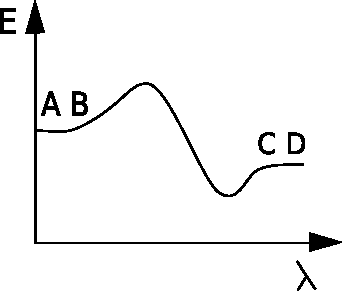
\includegraphics[height=5cm]{image/ElambdaRXN.pdf}
	\label{fig:E-lambda_RXN}
\end{figure}

dove $E$ indica l'energia, mentre $\lambda$ la coordinata di reazione.

\section{Ipotesi restrittive}
I fondatori della teoria dello stato di transizione sono Eyring\footnote{Chi era ....} e Polanyi\footnote{Polanyi, John C. (Berlino 1929), chimico canadese.} e basano le loro affermazioni sulle seguenti ipotesi:
\begin{itemize}
	\item \'E valida l'approssimazione di Born\footnote{Born, Max (Breslavia 1882 - Gottinga 1970), fisico britannico di origine tedesca.}-Hopenheimer\footnote{Dire chi era...}, ovvero: i moti elettromolecolari sono all'equilibrio ($v_{e^{-}} >> v_{nucleo}$)
	\item La distribuzione delle velocit� segue la legge di Maxwell\footnote{Maxwell, James Clerk (Edimburgo 1831 - Cambridge 1879), fisico britannico.}-Boltzman\footnote{Boltzmann, Ludwig (Vienna 1844 - Duino 1906), fisico austriaco}
	\item I sistemi che hanno superato lo stato di transizione non possono tornare indientro
	\item Vi � equilibrio tra reagenti e stato di transizione
	\item Nella prossimit� dello stato di transizione il moto lungo la coordinata di reazione � assimilabile ad una traslazione\\
		\begin{figure}[htbp]
			\centering
				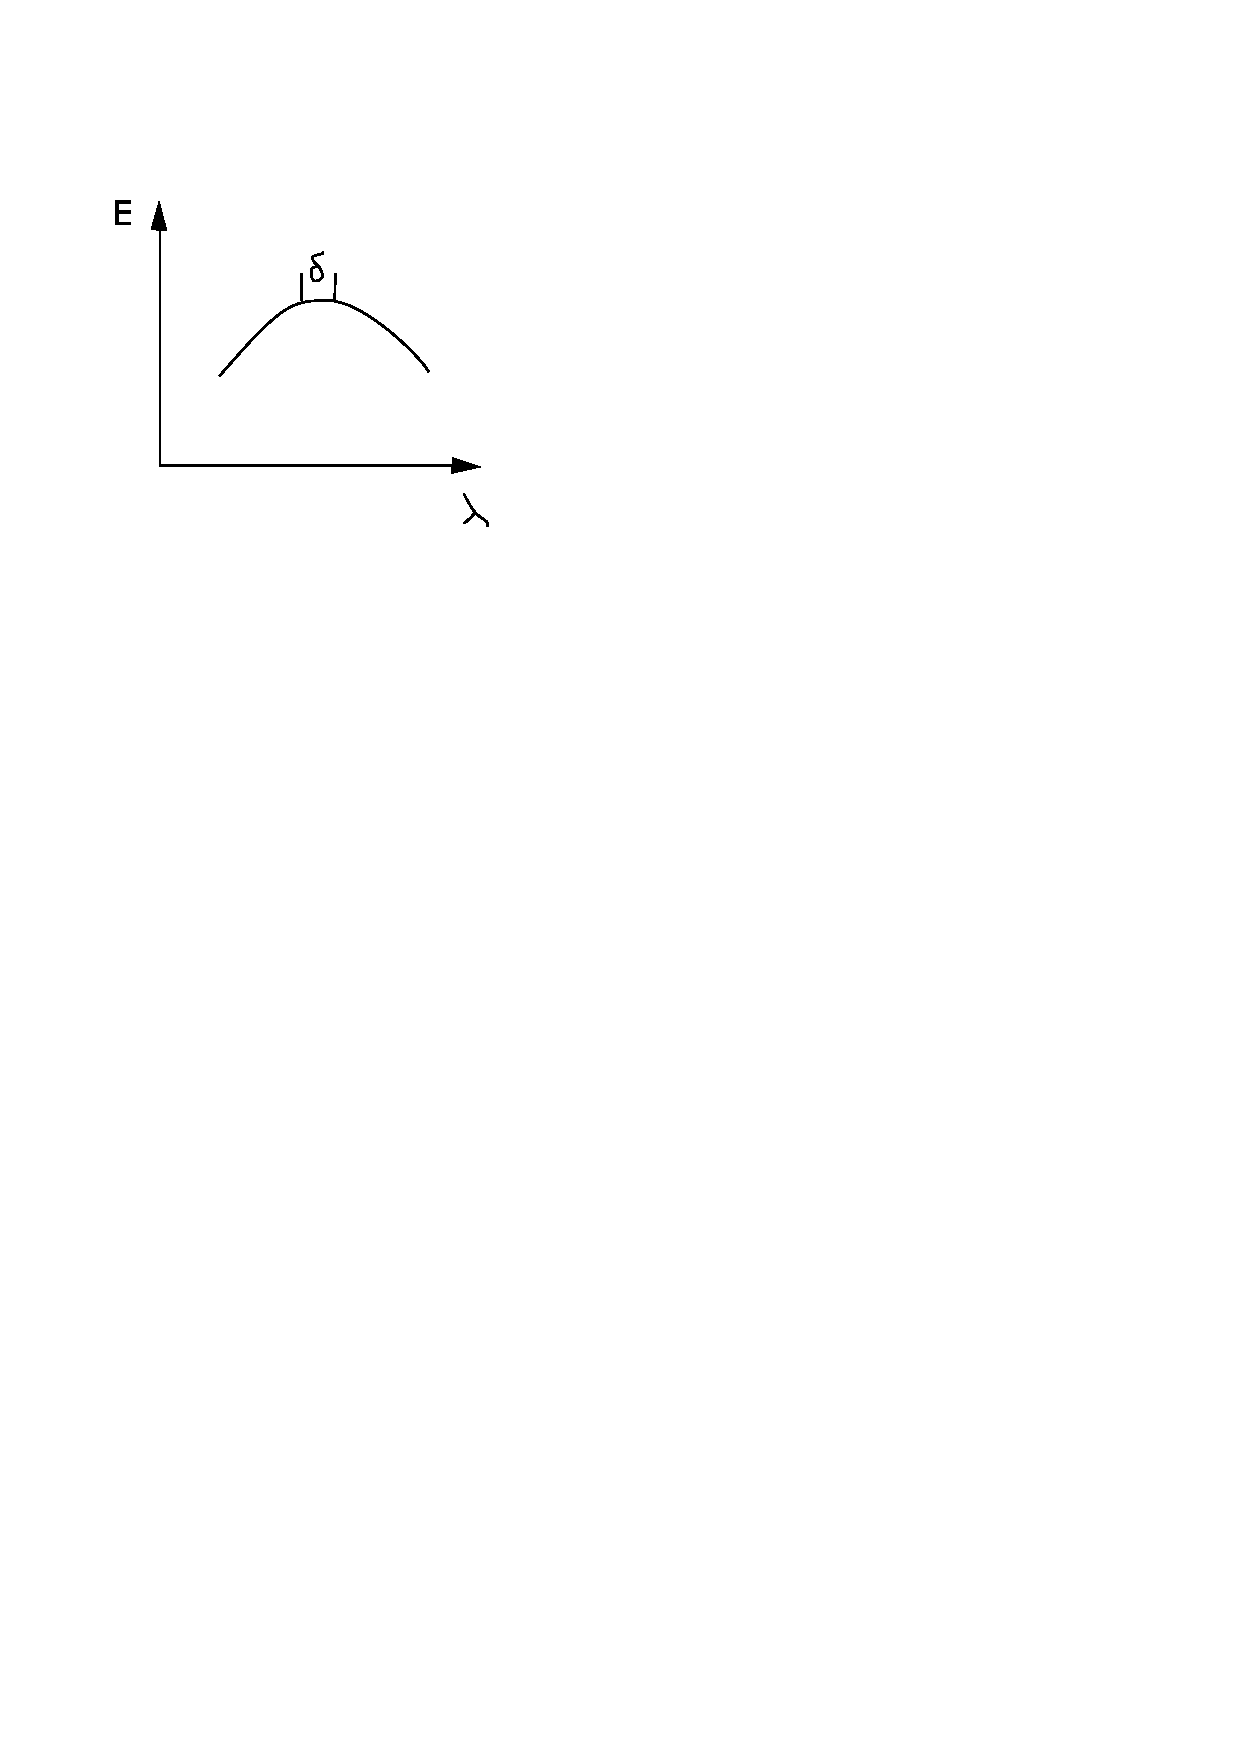
\includegraphics[height=3cm]{image/Delta_RXN.pdf}
			\label{fig:E-Delta_RXN}
		\end{figure}
\end{itemize}

Mentre la prime due ipotesi sono sempre verificate le successive sono ipotesi pi� restrittive, in particolare la terza � la pi� limitante.

\section{Velocit� di reazione}
Secondo quanto elencato qui sopra la reazione \ref{eq:ST:ReazioneGenerica} pu� essere vista come:
\begin{equation}
	A + B \rightleftharpoons X^{\ddagger} \rightarrow C + D
	\label{eq:ST:ReazioneIntermedioGenerica}
\end{equation}
Inoltre possiamo esprimere la velocit� di reazione come:
\begin{equation}
	R = C_{X^{\ddagger}} \cdot \frac{v^{\ddagger}}{\delta} \cdot \frac{1}{2}
	\label{eq:ST:VelocitaReazione}
\end{equation}
Dove $\delta$ � uno spessore arbitrario e $v^{\ddagger}$ � la velocit� della specie intermedia, che pu� essere espressa tramite la distribuzione di Boltzamn
\begin{equation}
	v^{\ddagger} = \sqrt{\frac{2 k_B \cdot T}{\pi m}}
	\label{eq:ST:VelocitaMaxwelBoltzman}
\end{equation}
che inserita nella velocit� di reazione (equazione \ref{eq:ST:VelocitaReazione}) porta a:
\begin{equation}
	R = C_{X^{\ddagger}} \cdot \frac{1}{2 \delta} \cdot \sqrt{\frac{2 k_B \cdot T}{\pi m}}
	\label{eq:ST:VelocitaReazioneMaxwelBoltzman}
\end{equation}

\subsection{Concentrazione della specie intermedia}
Cerchiamo ora di determinare $C_{X^{\ddagger}}$, sapendo che la reazione:
\begin{equation}
	A + B \rightleftharpoons X^{\ddagger}
	\label{eq:ST:ReazioneFormazioneIntermedio}
\end{equation}
si trova all'equilibrio, quindi la sua costante pu� essere espressa come:
\begin{equation}
	K_{eq} = \frac{C_{X^{\ddagger}}}{C_A \cdot C_B}
	\label{eq:ST:CostanteEquilibrioIntermedio}
\end{equation}
da cui si ottiene:
\begin{equation}
	C_{X^{\ddagger}}= K_{eq} \cdot C_A \cdot C_B
	\label{eq:ST:ConcIntermedioDaKeq}
\end{equation}
ed infine, sostituendo il risultato ottenuto nella \ref{eq:ST:VelocitaReazioneMaxwelBoltzman}, otteniamo:
\begin{equation}
	R =  K_{eq} \cdot C_A \cdot C_B \cdot \frac{1}{2 \delta} \cdot \sqrt{\frac{2 k_B \cdot T}{\pi m}}
	\label{eq:ST:VelocitaReazioneMaxwelBoltzmanKeq}
\end{equation}

\subsection{Costante di equilibrio in funzione della funzione di partizione molecolare}
Cerchiamo ora di correlare la costante di equilibrio con una funzione della \textsl{funzione di partizione molecolare}.

Ricordando dalla termodinamica che:
\begin{equation}
	G = F + P \cdot V
	\label{eq:ST:GTermodinamica}
\end{equation}
e anche 
\begin{equation}
	P \cdot V = n \cdot R \cdot T = n \cdot k_B \cdot N_A \cdot T = N \cdot k_B \cdot T
	\label{eq:ST:GasPerfetti}
\end{equation}
da questa otteniamo e dall'equazione precedente abbiamo:
\begin{equation}
	G = F +  N \cdot k_B \cdot T
	\label{eq:ST:GTermodinamicaGasPerfetti}
\end{equation}
ma dalla termodinamica statistica sappiamo che:
\begin{equation}
	F = - k_B \cdot T \cdot \ln z
	\label{eq:ST:FTermodinamicaStatistica}
\end{equation}
con $z$ \textsl{funzione di partizione}, da cui tornando all'equazione \ref{eq:ST:GTermodinamicaGasPerfetti}, ricaviamo:
\begin{equation}
	G = N \cdot k_B \cdot T - k_B \cdot T \cdot \ln z = k_B \cdot T (N - \ln z)
	\label{eq:ST:GTermodinamicaStatisticaGasPerfetti}
\end{equation}
poich�, per quanto visto precedentemente, per i gas perfetti � anche vero che:
\begin{equation}
	z = \frac{Q^N}{N!}
	\label{eq:ST:FunzParizMolecolare}
\end{equation}
otteniamo:
\begin{multline}
	G = k_B \cdot T (N - \ln \frac{Q^N}{N!}) = \\
			k_B \cdot T (N - \ln Q^N + \ln N!) =  \\
			k_B \cdot T (N - N \ln Q + N \ln N - N)
	\label{eq:ST:GFunzParizMolecolare}
\end{multline}
dove nell'ultimo passaggio � stata utilzzata l'approssimazione di Stearling\footnote{l'approssimazione di stearling dimostra che per $x$ elevati $\ln x! = x \ln x - x$}. Raccogliendo gli elementi e semplificando (considerando una sola mole di molecole) si ottiene:
\begin{multline}
	G = k_B \cdot T (N \ln N - N \ln Q) = \\
			- k_B \cdot T \cdot N (\ln Q - \ln N ) = \\
			- k_B \cdot T \cdot N \left(\ln \frac{Q}{N}\right) = \\
			- k_B \cdot T \cdot N_A \left(\ln \frac{Q}{N_A}\right) = \\
			- R \cdot T \ln \frac{Q}{N_A} 
	\label{eq:ST:GFunzParizMolecolareSemplificata}
\end{multline}

Dalla termodinamica sappiamo che:
\begin{equation}
	K_{eq} = e^{-\frac{\Delta \tilde{G}^0_R}{R \cdot T}}
	\label{eq:ST:KeqTermodinamica}
\end{equation}
dove
\begin{equation}
	\Delta \tilde{G}^0_R = \sum_i \nu_i \tilde{G}_{i\:(P,T)}
	\label{eq:ST:DGo}
\end{equation}
e dividendo ambo i membri per $R \cdot T$ ottengo:
\begin{equation}
	\frac{\Delta \tilde{G}^0_R}{R \cdot T} = \sum_i \nu_i \frac{\tilde{G}_{i\:(P,T)}}{R \cdot T}
	\label{eq:ST:DGoTR}
\end{equation}

Ricordando la definizione di $G$ ricavata prima (equazione \ref{eq:ST:GFunzParizMolecolareSemplificata}) per una mole abbiamo:
\begin{equation}
	\frac{\Delta \tilde{G}}{R \cdot T} = - \ln \frac{Q}{N_A}
	\label{eq:ST:GSuRTMoleTermoStat}
\end{equation}
da cui, inserendolo nell'equazione \ref{eq:ST:KeqTermodinamica} e logaritmando:
\begin{multline}
	\ln K_{eq} = - \frac{\Delta \tilde{G}^0_R}{R \cdot T} = 
							 - \sum_i \nu_i \frac{\tilde{G}_{i\:(P,T)}}{R \cdot T} = 
							 \sum_i \nu_i \ln\frac{Q}{N_A} = \\
							 \sum_i \ln \left(\frac{Q}{N_A}\right)^{\nu_i} = 
							 \ln \prod_i \left(\frac{Q}{N_A}\right)^{\nu_i}
	\label{eq:ST:LnKeqTermodinamicaStatistica}
\end{multline}
ed elevando ad esponente
\begin{equation}
	K_{eq} = \prod_i \left(\frac{Q}{N_A}\right)^{\nu_i}
	\label{eq:ST:LnKeqTermodinamicaStatistica}
\end{equation}

Ricordando dalla termodinamica statistiche il valore di $Q_{TRAS}$, sappiamo che:
\begin{equation}
	 Q_i = Q' \cdot V
	\label{eq:ST:QVTermoStat}
\end{equation}
quindi la costante di equilibrio risulter� essere:
\begin{equation}
	 K_{eq} = \prod \left( \frac{Q' \cdot V}{N_A} \right)^{\nu} = \prod (Q' \cdot \tilde{v})^{\nu}
	\label{eq:ST:KeqQV}
\end{equation}
essendo anche:
\begin{equation}
	 C_{TOT} = \frac{1}{\tilde{v}}
	\label{eq:ST:Ctot}
\end{equation}
abbiamo:
\begin{equation}
	K_{eq} = 	\frac{1}{C_{TOT}^{\sum_i \nu_i}} \prod_i Q'^{\nu_i} = 
						\prod_i \left( \frac{C_i}{C_0} \right)^{\nu_i} = 
						 \left( \frac{\prod_i C_i^{\nu_i}}{C_0^{\sum_i \nu_i}} \right)
	\label{eq:ST:KeqQCtot}
\end{equation}
e semplificando:
\begin{equation}
	\frac{\prod_i C_i^{\nu_i}}{C_0^{\sum_i \nu_i}} =
	\frac{\prod_i Q'^{\nu_i}}{C_{TOT}^{\sum_i \nu_i}}
	\label{eq:ST:KeqQCtotSemplif}
\end{equation}
da cui ottengo:
\begin{equation}
	\prod_i C_i^{\nu_i} =	\prod_i Q'^{\nu_i}
	\label{eq:ST:QCi}
\end{equation}
Ritornando all'equazione \ref{eq:ST:VelocitaReazioneMaxwelBoltzmanKeq} ottengo:
\begin{equation}
	R = C_A \cdot C_B \cdot \prod_i Q'^{\nu_i} \cdot \frac{1}{2 \delta} \cdot \sqrt{\frac{2 k_B \cdot T}{\pi m}}
	\label{eq:ST:VelocitaReazioneFinale}
\end{equation}
Da cui si evidenzia che la costante cinetica risulter� essere paria a:
\begin{equation}
	K_{CIN} = \prod_i Q'^{\nu_i} \cdot \frac{1}{2 \delta} \cdot \sqrt{\frac{2 k_B \cdot T}{\pi m}} = 
						\frac{1}{2 \delta} \cdot \sqrt{\frac{2 k_B \cdot T}{\pi m}} \cdot \frac{Q'_{\ddagger}}{Q_A \cdot Q_B}
	\label{eq:ST:VelocitaReazioneFinaleQ}
\end{equation}

\section{La costante cinetica}
Come si pu� vedere la costante cinetica dipende ancora dal parametro $\delta$ che essendo un parametro arbitrario deve essere rimosso. Per fare questo esplicitiamo $Q'_{\ddagger}$ ottenendo:
\begin{equation}
	K_{CIN} = \frac{1}{2 \delta} \cdot \sqrt{\frac{2 k_B \cdot T}{\pi m}} \cdot
						\frac{Q_{ROT}^{\ddagger} \cdot Q_{VIB}^{\ddagger} \cdot 
									Q_{TRAS}^{\ddagger} \cdot Q_{EL}^{\ddagger}}
								 {Q_A \cdot Q_B}
	\label{eq:ST:KcinFinaleQddagger}
\end{equation}
Il moto vibrazionale lungo la direzione delle coordinate di reazione degenera in un moto traslatorio, quindi otteniamo:
\begin{equation}
	K_{CIN} = \frac{1}{2 \delta} \cdot \sqrt{\frac{2 k_B \cdot T}{\pi m}} \cdot
						\frac{Q_{ROT}^{\ddagger}  \cdot Q_{EL}^{\ddagger} \cdot
									Q_{TRAS}^{\ddagger} \cdot (Q_{VIB-1}^{\ddagger} \cdot Q_{TRAS}^{\ddagger 1D})}
								 {Q_A \cdot Q_B}
	\label{eq:ST:KcinQddaggerDegenerato}
\end{equation}
ed essendo:
\begin{equation}
	Q_{TRAS}^{\ddagger 1D} = \sqrt{\frac{2 \pi m \cdot k_B \cdot T}{h^2}} \cdot L
	\label{eq:ST:Qdagger1D}
\end{equation}
ponendo $L = \delta$ e semplificando, otteniamo:
\begin{multline}
	K_{CIN} = \frac{1}{2} \cdot \sqrt{\frac{2 k_B \cdot T}{\pi m}} \cdot
						\sqrt{\frac{2 \pi m \cdot k_B \cdot T}{h^2}} \cdot
						\frac{Q_{ROT}^{\ddagger}  \cdot Q_{EL}^{\ddagger} \cdot
									Q_{TRAS}^{\ddagger} \cdot Q_{VIB-1}^{\ddagger}}
								 {Q_A \cdot Q_B} = \\
						\frac{k_B \cdot T}{h} \cdot
						\frac{Q_{ROT}^{\ddagger}  \cdot Q_{EL}^{\ddagger} \cdot
									Q_{TRAS}^{\ddagger} \cdot Q_{VIB-1}^{\ddagger}}
								 {Q_A \cdot Q_B}
	\label{eq:ST:KcinQddaggerDegenerato}
\end{multline}
La costante cinetica pu� anche essere esplicitata come:
\begin{multline}
	K_{CIN} =	\frac{k_B \cdot T}{h} \cdot
						\frac{Q_{ROT}^{\ddagger}  \cdot Q_{EL}^{\ddagger} \cdot
									Q_{TRAS}^{\ddagger} \cdot Q_{VIB-1}^{\ddagger}}
								 {Q_{ROT}^A  \cdot Q_{EL}^A \cdot	Q_{TRAS}^A \cdot Q_{VIB}^A \cdot 
									Q_{ROT}^B  \cdot Q_{EL}^B \cdot	Q_{TRAS}^B \cdot Q_{VIB}^B }
	\label{eq:ST:KcinEsplicitata}
\end{multline}
da cui raccogliendo i contributi elettronici:
\begin{multline}
	K_{CIN} =	\frac{k_B \cdot T}{h} \cdot
						\frac{Q_{ROT}^{\ddagger} \cdot Q_{TRAS}^{\ddagger} \cdot Q_{VIB-1}^{\ddagger}}
								 {Q_{ROT}^A \cdot	Q_{TRAS}^A \cdot Q_{VIB}^A \cdot 
									Q_{ROT}^B \cdot	Q_{TRAS}^B \cdot Q_{VIB}^B } \cdot
						\frac{Q_{EL}^{\ddagger}}{Q_{EL}^A \cdot	Q_{EL}^B} = \\
						\frac{k_B \cdot T}{h} \cdot
						\frac{Q_{ROT}^{\ddagger} \cdot Q_{TRAS}^{\ddagger} \cdot Q_{VIB-1}^{\ddagger}}
								 {Q_{ROT}^A \cdot	Q_{TRAS}^A \cdot Q_{VIB}^A \cdot 
									Q_{ROT}^B \cdot	Q_{TRAS}^B \cdot Q_{VIB}^B } \cdot
						e^{-\frac{\epsilon_{EL}^{\ddagger} - \epsilon_{EL}^A - \epsilon_{EL}^B}{k_B \cdot T}} =\\
						\frac{k_B \cdot T}{h} \cdot
						\frac{Q_{ROT}^{\ddagger} \cdot Q_{TRAS}^{\ddagger} \cdot Q_{VIB-1}^{\ddagger}}
								 {Q_{ROT}^A \cdot	Q_{TRAS}^A \cdot Q_{VIB}^A \cdot 
									Q_{ROT}^B \cdot	Q_{TRAS}^B \cdot Q_{VIB}^B } \cdot
						e^{-\frac{\Delta \epsilon_{EL}}{k_B \cdot T}}
	\label{eq:ST:KcinEsplicitataElettronici}
\end{multline}
Raccogliendo anche le $Q_{VIB}$ possiamo scrivere:
\begin{equation}
	\frac{Q_{VIB}^{\ddagger}}{Q_{VIB}^A \cdot Q_{VIB}^B} = 
	e^{- \frac{\sum \frac{h \nu^{\ddagger}}{2} - \sum \frac{h \nu^A}{2} - \sum \frac{h \nu^B}{2}}
						{k_B \cdot T}}
	\label{eq:ST:QVibrazRaccolte}
\end{equation}
l'esponente viene chiamato \textsl{$\Delta$ZPE\footnote{Zero Point Energy}} ovvero � l'energia che tutte le molecole possiedono allo stato $0$. La costante cinetica pu� essere riscritta, quindi, come:
\begin{equation}
	K_{CIN} =	\frac{k_B \cdot T}{h} \cdot
						\frac{Q_{ROT}^{\ddagger} \cdot Q_{TRAS}^{\ddagger}}
								 {Q_{ROT}^A \cdot	Q_{TRAS}^A \cdot Q_{ROT}^B \cdot Q_{TRAS}^B} \cdot
						e^{-\frac{\Delta(\epsilon_{EL} + ZPE)}{k_B \cdot T}}
	\label{eq:ST:KcinFin}
\end{equation}

Se confrontiamo l'equazione ottenuta con l'equazione di Arrenus si nota che le due equazioni sono identiche se si pone:
\begin{equation}
	\Delta E_{ATT} = \Delta(\epsilon_{EL} + ZPE)
	\label{eq:ST:ArreniusDEatt}
\end{equation}
\begin{equation}
	A = \frac{k_B \cdot T}{h} \cdot
			\frac{Q_{ROT}^{\ddagger} \cdot Q_{TRAS}^{\ddagger}}
					 {Q_{ROT}^A \cdot	Q_{TRAS}^A \cdot Q_{ROT}^B \cdot Q_{TRAS}^B}
	\label{eq:ST:ArreniusA}
\end{equation}
ottenendo quindi:
\begin{equation}
	K_{CIN} =	A \cdot e^{-\frac{\Delta E_{ATT}}{k_B \cdot T}}
	\label{eq:ST:KcinFin}
\end{equation}